\chapter{Struktura i sterowanie robotem}
\label{cha:strukturaISterowanie}

\section{Stanowisko}
\label{sec:stanowisko}

\subsection{Robot przmysłowy}
\label{sebsec:RobotPrzemyslowy}
\noindent Producent: Zakłady Automatyki Przemysłowej Ostrów Wielkopolski\\
Model: IRp-6\\
Parametry:\\
\begin{tabular}{|l|l|l|} \hline
\multicolumn{2}{|l|}{Osie sterowane: }& {5} \\ \hline
\multicolumn{2}{|l|}{Kontrolery: }& {USR-6}\\ \hline
\multicolumn{2}{|l|}{Maksymalne obciążenie: } & {6 kg}\\ \hline
\multicolumn{2}{|l|}{Powtarzalność: }& {+-0,20 mm}\\ \hline
\multicolumn{2}{|l|}{Masa jednostki mechanicznej: }& {125 kg}\\ \hline
\multicolumn{2}{|l|}{Zasięg: }& \\ \hline
{Zakres ruchu:} & {Oś1:} & {+- 160} \\ \cline{2-3}
& Oś2: & +- 40 \\ \cline{2-3}
& Oś3: & -25..+40\\ \cline{2-3}
& Oś4: & -25..+120\\ \cline{2-3}
& Oś5: & -25..+150\\ \hline
Prędkość maksymalna: & Oś1: & 60 \\ \cline{2-3}
& Oś2: & 60 \\ \cline{2-3}
& Oś3: & 60 \\ \cline{2-3}
& Oś4: & 75 \\ \cline{2-3}
& Oś5: & 125\\ \hline
%Moment: & Oś1: & \\ \cline{2-3}
%& Oś2: & \\ \cline{2-3}
%& Oś3: & \\ \cline{2-3}
%& Oś4: & \\ \cline{2-3}
%& Oś5: & \\ \hline
\end{tabular}

\vspace{5mm}

Podstawa robota została umieszczona na napędzie liniowym, w celu poszerzenia obszaru roboczego, tak aby pokrywał się on z polem widzenia systemu wizyjnego.\\
Parametry:\\
\begin{tabular}{|l|l|}\hline
Napęd: & Elektryczny napęd liniowy ze śrubą \\ \hline
Wielkość: & \\ \hline
Skok [mm]: & \\ \hline
Maks. siła podawania [N]: & \\ \hline
Moment My/Mz [Nm]: & \\ \hline
Moment Mx [Nm] & \\ \hline
Prędkość [m/s]: & \\ \hline
\end{tabular}
\subsection{Sterowanie}
Sterownie robotem odbywało się przez system modułowy dSpace DS1005. Komputer PC połaczony z tym systemem przez magistralę AT-bus, pełnił rolę prototypowania sterownika. W programie Matlab/Simulink utowrzony został sterownik robota, który przekonwetowany na kod źródłowy w języku C przez narzędzie RTW (Real-Time Workshop), został skopmilowany, zlinkowany oraz wgrany do karty procesowej DS1005 z procesorem sygnałowym za pomocą modułu RTI (Real-Time Interface). Ponadto uruchomiony w komputerze progrm ControlDesk, był interface'm graficznym  między sterownikiem a użytkownikiem, działającym w czasie pracy robota. Za pomocą tego programu wprowadzano potrzebne parametry do odpowiedniej pracy robota.


\noindent 
Komputer klasy PC\\
System operacyjny: Windows 2000 Serwer\\
Procesor:\\
Pamięć RAM:\\

\noindent Oprogramowanie:
\begin{itemize}
\item Matlab 2007b z bibliotekami: Simulink (służący do prototypowania sterownika), Iamge Prcessing Toolbox (do przetwarzania obrazu) oraz RTW (generacji kodu źródłowego z modelu Simulink) ;
\item Program ControlDesk - interface graficzny między operatorem, a sterownikiem;
\item Moduł RTI (Real-Time Interface) - służący do komunikacji z systemem dSpace.
\end{itemize}

System dSpace DS 1005 zawierał nastepujące karty:
\begin{itemize}
\item karta Master DS1005 - głowna jednostka obliczeniowa
\item karta Multi I/O DS2201 - wielofunkcyjna karta pomiarowa
\item karta wyjść analogowych DS2103
\item karta DS3001 - zliczanie impulsów z enkoderów
\end{itemize}

\subsection{System wizyjny}
\noindent Producent:\\
Model:\\
Parametry:\\
\noindent \begin{tabular}{|l|l|} \hline
{Rozdzielczość: }& \\ \hline
{Szybkość: } &\\ \hline
{Ilość klatek na sekundę: }&\\ \hline
{Pole widzenia: }&\\ \hline
{Formaty obrazu: }& \\ \hline
{Oświetlenie: }& {brak} \\ \hline
\end{tabular}
\subsection{Inne}
\noindent Stół o wymiarach:\\
\begin{tabular}{|l|l|}\hline
Wysokość: & 0,72 m\\ \hline
Szerokość: & 0,8 m\\ \hline
Długość: & 1,2 m\\ \hline
\end{tabular}
\newpage
\section{Model sterownika w simulinku}
\label{sec:modelWSimulinku}

\subsection{Serwomechanizm}
\label{subsec:Serwomechanizm}

Sterowanie napędów zostało zrealizowane przez zamknięty układ sterowania, przedstawionym na poniższym schemacie. %Wejściem układu było położenie kątowe złącza.

%
\begin{figure}
\centering
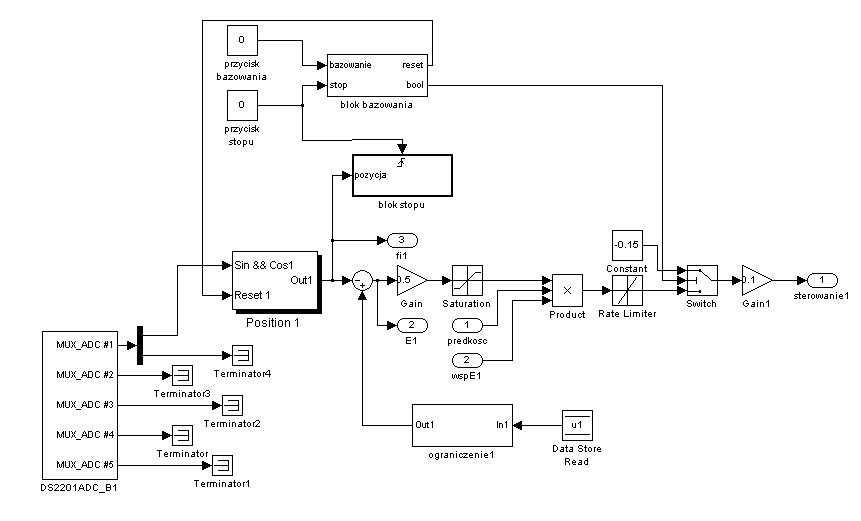
\includegraphics[width=16cm] {dodatki/zamkiety_ukl_reg_wyciete.jpg}
\caption{Schemat zamkniętego układu redulacji}
\label{fig:zamkiety_ukl_reg_wyciete}
\end{figure}

W~badanym przypadku zamknięcie sprzężenia zwrotnego odbywało się poprzez odczyt położenia kątowego z czujników umieszczonych w złączu. Dane te zostały odczytane przez moduł dSpace, a następnie poprzez blok DS2201ADC\_B1 zostały przekazane do modelu. Do sterowania wykorzystano regulator proporcjonalny. Ponieważ dla tego robota były realizowane zadania nadążąnia i~przestawiania, nie zastosowano członu całkującego, który zmiejszyłby zapas stabilności. Wartość współczynnika wzmocnienia została ustalona na podstawie przeprowadzonych eksperymtów opisanych w pozycji [?]. %zapytać z której publikacij wziąć nastawy P
Sygnał sterujący był odpowiednio przetworzony przez następujące operacje:
\begin{itemize}
\item ograniczenie sygnału (blok saturation) - silnik jak każdy obiekt rzeczywisty miał ograniczone wartości sterowania.
\item {} zamiana uchybu położenia na prędkość {} (blok mnożenia) - w zespole napędowym każdego złącza był silnik DC, w którym można sterować jego prędkością.
\item ograniczenie narastania sygnału (blok rate-limiter) - nie można było dopuścić do skokowej zmiany prędkości silnika, która mogłaby go uszkodzić.
\item normalizacja (blok gain2) -  karta DS2201 wymagała sygnału z przedziału (-0.3; 0.3)
\end{itemize}
Dodatkowo wartość zadana była ograniczana (blok ograniczenia..), ze względu na zakresy ruchu każdej osi podane w rozdziale \ref{sebsec:RobotPrzemyslowy}.
Blok ``Position .. `` konwertuje sygnał z czujnika na położenie podane w stopniach.

\noindent Parametry wejsciowe subsystemu:
\begin{itemize}
\item``pomiar.. `` - sygnał z czujnika położenia
\item ``predkosc `` - zadana prędkość podana w \%
\end{itemize}
\noindent Parametry wejsciowe subsystemu:
\begin{itemize}
\item ``sterowanie.. `` - sygnał sterujący silnikiem w~danym złączu 
\end{itemize}

\begin{figure}
\centering
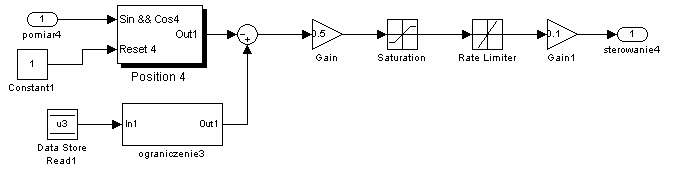
\includegraphics[width=16cm] {dodatki/bez_dodatkow2_wyciete.jpg}
\caption{Schemat serwomechanizmu bez dodatków}
\label{fig:bez_dodatkow2_wyciete}
\end{figure}

\subsection{Stop}
\label{subsec:Stop}

Zatrzymanie robota w dowolnym monencie było niezbędną częścią sterownika. Ta funkcja umożliwiała uniknięcie uszkodzenia robota lub innych przedmiotów w obszarze roboczym w przypadku awarii lub błedu operatora. To zadanie zrealizowano poprzez jednokrotne przypisanie aktualnego położenie do pozycji zadanej przez co uchyb ustalony zmniejszał się do zera i w efekcie sterowanie także się redukowało. W przypadku zatrzymania nie można było przypisać wprost zera do sterowania, ponieważ przerwałoby się pętle sprzężenia zwrotnego co skutkowałoby utratą kontroli.

\begin{figure}
\centering
\subfloat[stop]{\label{stop_wyciete}
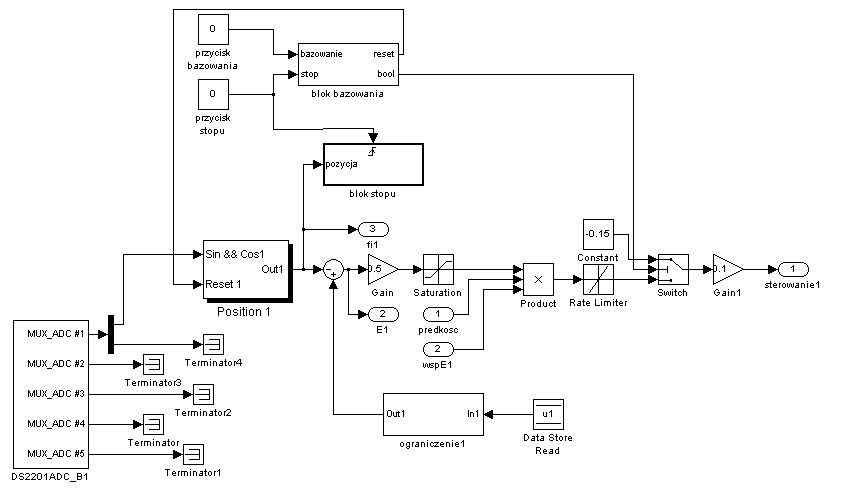
\includegraphics[width=0.7\textwidth]{dodatki/stop_wyciete.jpg}}
\quad
\subfloat[subsystem: blok stopu]{\label{stop_wyciete2}
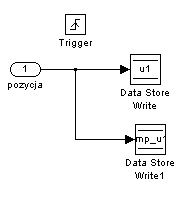
\includegraphics[width=0.2\textwidth]{dodatki/stop_wyciete2.jpg}}
\caption{Mechanizm stopu}
\label{fig:mechanizm_stopu}
\end{figure}

Jednorazowe przypisanie do wartości zadanej zrealizowano poprzez subsystem wyzwalany zboczem rosnącym.

\subsection{Sterowanie prędkością}
\label{subsec:sterowaniePredkoscia}

Operator mógł sterować prędkością poprzez zadawanie jaka część szybkości maksymalnej miałbyć wykorzystany. Wybrany procent wybranej prędkości był mnozony przez wartość sterowania regulatora. Nie można było podać do toru sterowania konkretnej szybkości, ponieważ skutkowałoby nieprawidłowym działaniem regulatora.

\subsection{Koordynacja ruchowa}
\label{subsec:koordynacjaRuchowa}

W sterowniku zaimplementowano koordynację ruchową (quasiliniowo). Celem jej działania było, żeby wszystkie zespoły napędowe rozpoczynały i kończyły wykonywanie ruchu w tym samym momencie. Zrealizowano to według poniższego algorytmu.
\begin{enumerate}
\item Wyznaczenie modułu błędu dla każdego złącza |epsi|
\item Znalezienie maksymalnego modułu błędu max|eps|
\item Wyznaczenie współczynnika prędkości dla każdej osi wsp = |epsi|/max|eps|
\item Ograniczenie wyliczonego współczynnika wsp do przedziału (0;1] 
\item Pomnożenie wartości wzmocnienia przez wsp.
\end{enumerate}
Poniżej przedstawiono model działania tej operacji.
%i

\begin{figure}
\centering
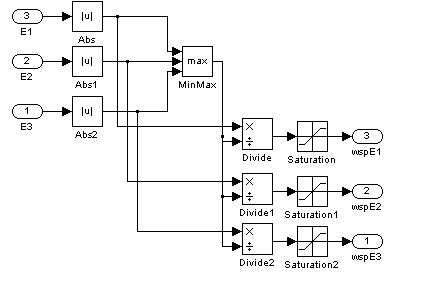
\includegraphics[width=12cm] {dodatki/quasiliniowosc_p2_wyciete.jpg}
\caption{Schamet quasiliniowości}
\label{fig:schamet_quasiliniowosci}
\end{figure}
Wejścia E1, E2, E3 zawierały różnicę między wartością zadaną, a wartością aktualną. Natomiast wyjścia wspE1, wspE2, wspE3 są podowane do serwomechanizmu jako mnożnik prędkości.

\subsection{Bazowanie}
\label{subsec:Bazowanie}

Czujniki położenia działały na zasadzie pomiaru różnicy od wartości początkowej. Do ich prawidłowego działania należało zaraz po włączeniu robota ustawić go w~określonej pozycji. W~tym celu w~każdym złączu znajdowały się cyfrowe czujniki położenia bazowego. Do bazowania wykorzystano następujący algorytm:
\begin{enumerate}
\item Ręczne wysterowanie robota, tak aby się znalazł w~pozycji przedbazowej tzn. każde złącze znajdowało się w obszarze między czujnikiem bazowania, a położeniem skrajnym.
\item Zadanie małej prędkości na każdy zespół napędowy w kierunku czujnika bazowania.
\item W~chwili dotarcia do pozycji bazowej zatrzymanie złącza.
\item Po ustawieniu każdego ramienia w~pozycji bazowej, zresetowanie czujników położenia.
\end{enumerate}
Powyższy algorytm został zrealizowany w Simulinku w następujący sposób.

\begin{figure}
\centering
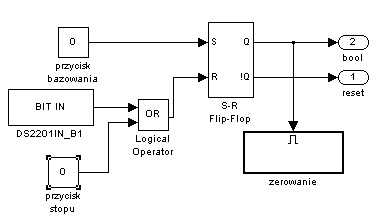
\includegraphics[width=12cm] {dodatki/bazowanie_p1_wyciete.jpg}
\caption{Schemat bazowania}
\label{fig:schemat_bazowania}
\end{figure}
W bloku zerowanie, wartość 0 została przypisana do odpowiednich zmiennych. 

Do wykonania tej operacji wykorzystano przerzutnik SR. Sygnał z przycisku rozpoczynającego bazowanie został podłączony do wejścia SET. Natmiast alternatywa odczytu z cyfrowego czujnika położenia i przycisku Stop do wejścia RESET. Zastosowanie tej operacji dawało kontrolę nad robotem w przypadku awarii. Zgodnie z zasadą działania przerzutnika po chwilowym pojawieniu się sygnału z przycisku rozpoczęcia bazowania wartość Q została ustawiona na 1. Ten sygnał został doprowadzany do przełącznika, który ustawił odpowiednie sterowanie. Kiedy złącze doszło do pozycji bazowej, odczyt z czujnika bazowego zminił się na 1 i wtedy sygnałem z wyjścia !Q czujnik położenia został zresetowany, a silnik zatrzymany.

\section{Przestrzeń robocza}
\label{sec:przestrzen_robocza}

Jak wspomniano w \ref{subsec:RobotPrzemyslowy} podstawę manipulatora umieszczono na napędzie liniowym, co znacznie zwiększyło jego powierzchnię roboczą. 
Poniżej przedstawiono przestrzeń roboczą dla wysokości 865 mm dla robota IRp-6 bez dodatkowego złącza pryzmatycznego oraz z nim.


\section{Proste zadanie kinematyki}
\label{sec:proste_zad_kinematyki}

Niezbedne do sterowania robotem była zamiana współrzędnych złączowych na współrzędne kartezjańskie. W tym celu rozwiązano proste zadanie kinematyki. 
Ponieżej przedstawiono schemat łańcucha kinematycznego, razem z wyznaczonymi układami współrzędnych złączowych według notacji Denavita-Hartenberga. Jako początek głównego układu współrzędnych przyjęto miejsce przecięcia się osi środkowej z podłożej, w pozycji bazowej robota.
%Schemat z Worda
\begin{table}[h]
\begin{center}
\begin{tabular}{r|c c c c}
   & $\alpha$ 	& a 		& d 		& $\Theta$ 			\\ \hline
1 & $\pi/2$ 	& 0 		& $d_1$ 	& 0 					\\
2 & $\pi/2$ 	& 0 		& $p_1$ 	& $\Theta_2+\pi/2$ 	\\
3 & 0 		& $p_2$ 	& 0  	& $\Theta_3+\pi/2$ 	\\
4 & 0 		& $p_3$ 	& 0 		& $\Theta_4-\pi/2$ 	\\
5 & $-\pi/2$ 	& 0		& 0 		& $\Theta_5$			\\
6 & 0 		& 0 		& $p_4$	& $\Theta_6-\pi/2$		\\
\end{tabular}
\caption{Parametry złączy}
\end{center}
\end{table}

Macierze przekształcenia dla poszczególnych złączy:

\vspace{5mm}

$A_1 = 
\begin{bmatrix}
1 		& 0 		& 0 		& 0 		\\
0 		& 0 		& -1		& 0 		\\
0 		& 1		& 0 		& d_1	\\
0 		& 0 		& 0 		& 1 		\\
\end{bmatrix}$
$A_2 = 
\begin{bmatrix}
-\sin \Theta_2		& 0 		& -\sin \Theta_2	& 0 		\\
\cos \Theta_2		& 0 		& \cos \Theta_2	& 0 		\\
0 				& 1 		& 0 				& p_1	\\
0 				& 0 		& 0 				& 1 		\\
\end{bmatrix}$
$A_3 = 
\begin{bmatrix}
-\sin \Theta_3 	& -\cos \Theta_3	& 0 		& -p_2\sin \Theta_3 	\\
\cos \Theta_3		& -\sin \Theta_3	& 0 		& p_2\cos \Theta_3 	\\
0 				& 0 				& 1 		& 0 					\\
0 				& 0 				& 0 		& 1 					\\
\end{bmatrix}$

$A_4 = 
\begin{bmatrix}
\sin \Theta_4 		& \cos \Theta_4	& 0 		& p_3\sin \Theta_4 	\\
-\cos \Theta_4	& \sin \Theta_4 	& 0 		& -p_3\cos \Theta_4 	\\
0 				& 0 				& 1 		& 0 					\\
0 				& 0 				& 0 		& 1 					\\
\end{bmatrix}$
$A_5 = 
\begin{bmatrix}
\cos \Theta_5		& 0 		& -\sin \Theta_5	 & 0 		\\
\sin \Theta_5	 	& 0 		& \cos \Theta_5 	& 0 		\\
0 				& -1 	& 0 				& 0 		\\
0 				& 0 		& 0 				& 1 		\\
\end{bmatrix}$
$A_6 = 
\begin{bmatrix}
\sin \Theta_6	 	& \cos \Theta_6	& 0 		& 0 		\\
-\cos \Theta_6	& \sin \Theta_6	& 0 		& 0 		\\
0 				& 0 				& 1 		& p_4	\\
0 				& 0 				& 0 		& 1 		\\
\end{bmatrix}$

\vspace{5 mm}

Macierz przekształcenia:

$T_0^6=
\begin{bmatrix}
t_{11}		& t_{12}	& t_{13}	& t_{14}	\\
t_{21}		& t_{22}	& t_{23}	& t_{24}	\\
t_{31}		& t_{32}	& t_{33}	& t_{34}	\\
0		& 0		& 0		& 1	\\
\end{bmatrix}$

\vspace{5 mm}

$t_{11} = \cos \Theta_2 \cos \Theta_6 - \sin \Theta_6 (\cos \Theta_5 (\cos \Theta_3 \cos \Theta_4 \sin \Theta_2 - \sin \Theta_2 \sin \Theta_3 \sin \Theta_4) - \sin \Theta_5 (\cos \Theta_3 \sin \Theta_2 \sin \Theta_4 + \cos \Theta_4 \sin \Theta_2 \sin \Theta_3))$
$t_{12} = $
$t_{13} = $
$t_{14} = $
$t_{21} = $
$t_{22} = $
$t_{23} = $
$t_{24} = $
$t_{31} = $
$t_{32} = $
$t_{33} = $
$t_{34} = $

Na podstawie wyliczononej macierzy przeszktałceń można było zapisać funkcje wyznaczające współrzędne końcówki roboczej w układzie kartezjańskim:

\noindent
$x = dd \\
y = gg \\
z = hh \\$

\newpage
\section{Odwrotne zadanie kinematyki}
\label{sec:odwrotneZadanieKinematyki}

Uwzglęniając złączę pryzmatyczne, na której została zainstalowana podstawa robota, układ wykonawczy miał 6 stopni swobody. Dwa ostatnie złacza służyły do ustawienia orientacji chwytaka tak, aby był on zawsze skierowany pionowo w dół. W tym przypadku łańcuch kinematyczny ustawiający położenie końcówki robota miał 4 stopnie swobody, oznacza że był redundatny (posiadał więcej stopni swobody niż ilości zmienych koniecznych do opisania położenia). Z tego wynikało, że rozwiązanie odwrotnego zadania kinematyki nie jest jednoznaczne. Robot mógł dojść do zadanej pozycji na więcej niż jeden sposób. Z tego powodu opracowano algorytm obliczania zmiennych złączowych ze współrzędnych kartezjańskich docelowej pozycji końcówki roboczej.
%Schemat algorytmu

W powyższym algorytmie zminimalizowano użycie napędu liniowego, ponieważ w porównaniu do innych złączy jest wolny (2 m/s).
